\documentclass[11pt]{article}

\usepackage[a4paper]{geometry}
\geometry{left=2.0cm,right=2.0cm,top=2.5cm,bottom=2.5cm}

% Chinese support
\usepackage{ctex}

% Math packages
\usepackage{amsmath,amsfonts,amssymb,amsthm,bm,mathrsfs,mathtools,breqn}

% Graphics and Colors
\usepackage{graphicx}
\usepackage{xcolor}
\usepackage{tikz}
\usetikzlibrary{arrows.meta,positioning}
\usepackage{pgfplots}
\pgfplotsset{compat=1.18}
\usepackage{circuitikz}
\graphicspath{{fig/}}

% Units
\usepackage{siunitx}

% Algorithms
\usepackage{algorithm}
\usepackage[noend]{algpseudocode}

% Layout and formatting
\usepackage{fancyhdr}
\usepackage[framemethod=TikZ]{mdframed}
\usepackage{fontspec}
\usepackage{fontsize}
\usepackage{adjustbox}
\usepackage{float}
\usepackage{multicol}
\usepackage{multirow}
\usepackage{pdfpages}
\usepackage{wrapfig}
\usepackage{subcaption}
\usepackage[inline]{enumitem}

% Tables
\usepackage{booktabs}
\usepackage{bigstrut,rotating}

% Listings
\RequirePackage{listings}

% Hyperlinks
\usepackage{hyperref}
\hypersetup{colorlinks=true,linkcolor=blue}

% Cross-referencing
\usepackage[capitalize]{cleveref}
\Crefname{section}{Section}{Sections}
\Crefname{table}{Table}{Tables}
\crefname{table}{Table.}{Tabs.}

% Listing settings
\definecolor{dkgreen}{rgb}{0,0.6,0}
\definecolor{gray}{rgb}{0.5,0.5,0.5}
\definecolor{mauve}{rgb}{0.58,0,0.82}

\lstset{
  frame=tb,
  aboveskip=3mm,
  belowskip=3mm,
  showstringspaces=false,
  columns=flexible,
  framerule=1pt,
  rulecolor=\color{gray!35},
  backgroundcolor=\color{gray!5},
  basicstyle={\small\ttfamily},
  numbers=none,
  numberstyle=\tiny\color{gray},
  keywordstyle=\color{blue},
  commentstyle=\color{dkgreen},
  stringstyle=\color{mauve},
  breaklines=true,
  breakatwhitespace=true,
  tabsize=3,
}

\setmainfont{Palatino Linotype}
\setCJKmainfont{SimSun}[BoldFont=SimHei, ItalicFont=KaiTi]
\setCJKsansfont{SimHei}
\setCJKmonofont{FangSong}
\punctstyle{kaiming}
% 偏好的几个字体, 可以根据需要自行加入字体ttf文件并调用

% Restore standard emphasis to avoid requiring an undefined environment (kaishu).
% The original redefinition used an environment `kaishu` which is not defined
% in a default ctex setup and causes compilation errors. Use \textit for
% emphasis which works across engines.
\renewcommand{\emph}[1]{\textit{#1}}

%改这里可以修改实验报告表头的信息
\newcommand{\experiName}{温度测量}
\newcommand{\supervisor}{梁淼}
\newcommand{\name}{邓思豪}
\newcommand{\studentNum}{2023K8009909008}
\newcommand{\class}{3}
\newcommand{\group}{01}
\newcommand{\seat}{5}
\newcommand{\dateYear}{2025}
\newcommand{\dateMonth}{11}
\newcommand{\dateDay}{26}
\newcommand{\room}{西实204}
\newcommand{\others}{$\square$}


\begin{document}



\begin{center}
    \LARGE \bf 《\, 基\, 础\, 物\, 理\, 实\, 验\, 》\, 实\, 验\, 报\, 告
\end{center}

\begin{center}
    \noindent \emph{实验名称}\underline{\makebox[25em][c]{\experiName}}
    \emph{指导教师}\underline{\makebox[8em][c]{\supervisor}}\\
    \emph{姓名}\underline{\makebox[6em][c]{\name}} 
    % 如果名字比较长, 可以修改box的长度"6em"
    \emph{学号}\underline{\makebox[10em][c]{\studentNum}}
    \emph{分班分组及座号} \underline{\makebox[5em][c]{\class \ -\ \group \ -\ \seat }\emph{号}} （\emph{例}:\, 1\,-\,04\,-\,5\emph{号}）\\
    \emph{实验日期} \underline{\makebox[3em][c]{\dateYear}}\emph{年}
    \underline{\makebox[2em][c]{\dateMonth}}\emph{月}
    \underline{\makebox[2em][c]{\dateDay}}\emph{日}
    \emph{实验地点}\underline{{\makebox[6em][c]\room}}
    \emph{调课/补课} \underline{\makebox[3em][c]{\others\ 是}}
    \emph{成绩评定} \underline{\hspace{5em}}
    {\noindent}
    \rule[8pt]{17cm}{0.2em}
\end{center}

\section{实验目的}
\begin{enumerate}
    \item 用电位差计测热电偶的温差电动势。
    \item 学会电桥的使用，用平衡电桥测热敏电阻和铜电阻的温度特性曲线。
    \item 设计非平衡电桥实现对热敏电阻的实时测量。
\end{enumerate}

\section{实验仪器与用具}
本实验采用DHT-2型热学实验仪进行温度计的控温，里面装有热电偶温度计、铜电阻温度计、热敏电阻温度计，通过加热丝升温，通过风扇降温，可以用来测试不同类型温度计的温度特性曲线，确定温度系数等。

热电偶的电压通过UJ36a型携带式直流电位差计进行测量。电阻型温度计的电阻通过电桥进行测量，实验中所用的DHQJ-5型教学用多功能电桥具有开放式电桥、双臂电桥、单臂电桥、功率电桥及非平衡使用的单臂电桥等功能，可以用平衡电桥测温度计的电阻，用非衡电桥对温度计进行实时测量。

实验装置实物图如图1所示。中间是DHT-2型热学实验仪，下面是温控仪，上面是加热炉，温度计装在加热炉中。左边是电桥，用来测温度计的电阻值；右边是电位差计，用来测热电偶的电势；保温瓶中装的是冰水混合物，用作热电偶的低温端。

\begin{figure}[H]
    \centering
    
\includegraphics[width=0.8\textwidth]{fig1.png}
    \caption{温度测量装置实物图}
\end{figure}

\subsection*{1. DHT-2 热学实验装置温控仪}
控温仪前面板如图2所示。

\begin{figure}[H]
    \centering
    
\includegraphics[width=0.8\textwidth]{fig2.png}
    \caption{温控仪前面板}
\end{figure}

温控仪各接口定义如下：
\begin{enumerate}
    \item 测量值：显示器（绿）
    \item 设定值：显示器（红）
    \item 加数键（$\blacktriangle$）：在温度设定时，作加数键。
    \item 减数键（$\blacktriangledown$）：在温度设定时，作减数键。
    \item 设定键（S）：设定值：按设定键（S），SV显示器一位数码管闪烁，则该位进入修改状态，再按S键，闪烁位向左移一位，不按设定键（S）8秒（即数码管闪烁8秒）自动停止闪烁并返回至正常显示设定值。
    \item 设定键（S）+ 加数键（$\blacktriangle$）：组合键设定PID参数。
    \item 设定键（S）+ 减数键（$\blacktriangledown$）：组合键设定PID参数。
    \item[6-7.] 热电偶输出端子。
    \item[10.] 加热电流输出插座
    \item[12.] 加热炉信号输入插座
    \item[14.] 加热电流输出控制开关
    \item[8-9.] 热敏电阻输出端子(NTC)
    \item[11.] 风扇电压输出插座
    \item[13.] 加热电流调节电位器
    \item[15.] 加热电流显示表。
\end{enumerate}

使用时依次将“信号输入”、“风扇电压”、“加热电流”依次与上面的加热炉上面的接口相连，然后插好电源线，打开电源开关。

按设定键（S）选择温度的位数，按上下键加减数值，不按设定键（S）8秒，自动停止闪烁并返回至正常显示设定值。设定好加热温度后，将面板上的加热电流开关打开，加热炉座上的电风扇的电源开关关断。设定的温度低于$60^\circ C$时，加热电流最好小于1A，设定的温度高于$100^\circ C$时，加热电流最好调到最大。

实验做完，或者需要降温时，首先设置所需温度，将加热炉的支撑杆向上抬升，打开风扇，待温度降至室温或者设定值时，关闭风扇，降下支撑杆。

\subsection*{2. UJ36a型携带式直流电位差计}

\begin{figure}[H]
    \centering
    
\includegraphics[width=0.8\textwidth]{fig3.png}
    \caption{电位差计补偿法电路图}
\end{figure}

图3中各符号含义：
\begin{itemize}
    \item $E$ —— 工作电源
    \item $E_N$ —— 标准电池的电动势
    \item $E_x$ —— 被测电动势（或电压）
    \item $G$ —— 检流计
    \item $R_p$ —— 工作电流调节电阻
    \item $R$ —— 被测量电动势的补偿电阻
    \item $R_N$ —— 标准电池电动势补偿电阻
    \item $K$ —— 转换开关
\end{itemize}

UJ36a 型携带式直流电位差计，可以在实验室、车间现场和野外工作，能很方便地以补偿法原理，测量直流电压（或电动势）和对各种直流毫伏表及电子电位差计进行刻度校正。仪器另一主要用途，是配合各种测量温度的热电偶，能快速而准确地检测温度。

% 图片位置: 图4 电位差计操作面板

操作面板定义如下：
\begin{enumerate}
    \item[(1)] 未知电压测量接线柱
\begin{figure}[H]
    \centering
    
\includegraphics[width=0.8\textwidth]{fig4.png}
    \caption{电位差计操作面板}
\end{figure}
    \item[(2)] 倍率开关
    \item[(3)] 步进盘（规盘）
    \item[(4)] 电键开关
    \item[(5)] 检流计
    \item[(6)] 检流计调零
    \item[(7)] 工作电流调节变阻器
    \item[(8)] 滑线盘
\end{enumerate}

将K扳向标准位置，调节$R_p$，使检流计指零，这时标准电池的电动势由电阻$R_N$上的电压降补偿。
\begin{equation}
    E_N = I R_N
\end{equation}
式中：$I$ 是流过$R_N$和$R$的电流，称之为电位差计的工作电流。由(1)式可得：
\begin{equation}
    I = E_N / R_N
\end{equation}
工作电流调节好以后，将K板向“未知”位置，同时移动Q触头，再次使检流计指零，此时触头Q在R上的读数为$R_Q$，这时被测量的电动势或电压由电阻$R_Q$上的电压降补偿。
将(2)带入(3)得：
\begin{equation}
    E_x = I R_Q
\end{equation}
\begin{equation}
    E_x = \frac{R_Q}{R_N} E_N
\end{equation}
在实际的调节过程中，$R_Q$的调节用步进盘进行粗调，用滑线盘进行细调，为了读数方便，进行换算后直接标示电压值，而不是电阻值。

将待测电压接入后，将倍率开关拨到“$\times 1$”或者“$\times 0.1$”，调节“调零”旋钮将检流计调零；将“电键开关”拨到“标准”，调节工作电流调节变阻器，使检流计指零；将“电键开关”拨到“未知”，调节步进读数盘和滑线读数盘使检流计再次指零。未知电压读数为：
\begin{equation}
    U_x = (\text{步进盘读数} + \text{滑线盘读数}) \times \text{倍率}
\end{equation}
\begin{figure}[H]
    \centering
    
\includegraphics[width=0.6\textwidth]{fig5.png}
    \caption{单臂电桥原理电路图}
\end{figure}
\subsection*{3. DHQJ-5型教学用多功能电桥}
单臂电桥的电路原理图如图5所示。


\begin{table}[htbp]
    \centering
    \caption{单臂电桥技术参数和设定参考值}
    \begin{tabular}{ccccc}
        \toprule
        量程倍率 & 有效量程($\Omega$) & $R_1 (\Omega)$ & $R_2 (\Omega)$ & 工作电压 \\
        \midrule
        $10^{-3}$ & $1 \sim 11.111$ & 10000 & 10 & \\
        $10^{-2}$ & $10 \sim 111.11$ & 10000 & 100 & \\
        $10^{-1}$ & $100 \sim 1111.1$ & 10000 & 1000 & 3V \\
        $\times 1$ & $1K \sim 11.111K$ & 1000 & 1000 & \\
        $10$ & $10K \sim 111.11K$ & 1000 & 10000 & \\
        $10^2$ & $100K \sim 1111.1K$ & 100 & 10000 & 12V \\
        $10^3$ & $1M \sim 11.111M$ & 10 & 10000 & \\
        \bottomrule
    \end{tabular}
\end{table}
单臂电桥的技术参数和设定值如表1所示，本实验中平衡电桥所用的倍率为“$\times 1$”档，$R_1$和$R_2$的电阻值可以取1000欧，电压取3V。

电桥的面板如图6所示。

\begin{figure}[H]
    \centering
    
\includegraphics[width=0.8\textwidth]{fig6.png}
    \caption{多功能电桥操作}
\end{figure}操作，本实验中平衡电桥所用的倍率为“$\times 1$”档，$R_1$和$R_2$的电阻值可以取1000欧，电压取3V。

电桥的面板如图6所示。

% 图片位置: 图6 多功能电桥操作

平衡电桥测量步骤如下：
\begin{enumerate}
    \item 标准电阻$R_N$选择开关选择“单桥”档；
    \item 工作方式开关选择“单桥”档；
    \item 电源选择开关建议按表1有效量程选择工作电源电压；
    \item G开关选择“G内接”；
    \item 根据$R_x$值估计值，按表1选择量程倍率，设置好$R_1$、$R_2$值和$R_3$值，将未知电阻$R_x$接入$R_x$接线端子。（注意$R_x$端子上方短接片应接好）
    \item 打开仪器市电开关、面板指示灯亮；
    \item 建议选择毫伏表作为仪器检流计，释放“接入”按键，量程置“20mV”档，调节“调零”电位器，将数显表调零。调零后将量程转入200mV量程，按下“接入”按键，也可以选择微安表作检流计。
    \item 调节$R_3$各盘电阻，粗平衡后，可以选择200mV或20mV档，细调$R_3$位，使电桥平衡。
\end{enumerate}
由此可见，用平衡电桥测电阻时每步都需要调节$R_3$使检流计指零，适合测量温度计稳定后的电阻值，不能实时测量，动态反应温度的变化。

非平衡电桥是单臂电桥在非平衡状态下的一种工程应用，当外界温度、压力等物理量发生变化时，相应的电阻性传感应器电阻值发生变化，电桥就从平衡状态（预调平衡）变成不平衡状态，检流计测量的电压变化表征电阻传感器电阻值变化，从而间接测量出相应物理变化。
DHQJ-5 在非平衡使用时，其操作步骤基本同单臂电桥，但测量目的和测量方法有很大差异，在本实验中将使用非平衡电桥电压的变化线性表示热敏电阻温度计温度的变化。

\section{实验原理}

\subsection{用电位差计测热电偶的温差电动势}
热电偶亦称温差电偶，是由A、B两种不同材料的金属丝的端点彼此紧密接触而组成的。当两个接点处于不同温度时（如图7），在回路中就有直流电动势产生，该电动势称温差电动势或热电动势，测试电路如图8所示。当组成热电偶的材料一定时，温差电动势$E_x$仅与两接点处的温度有关，并且两接点的温差在一定的温度范围内有如下近似关系式：
\begin{equation}
    E_x \approx \alpha(t-t_0)
\end{equation}
式中$\alpha$称为温差电系数，对于不同金属组成的热电偶，是不同的，其数值上等于两接点温度差为$1^\circ C$时所产生的电动势。

\begin{figure}[H]
    \centering
    
\includegraphics[width=0.6\textwidth]{fig7.png}
    \caption{热电偶原理示意图}
\end{figure}

\begin{figure}[H]
    \centering
    
\includegraphics[width=0.6\textwidth]{fig8.png}
    \caption{热电偶测试电路}
\end{figure}

\begin{figure}[H]
    \centering
    
\includegraphics[width=0.6\textwidth]{fig9.png}
    \caption{热电偶温度计测温原理}
\end{figure}

为了测量温差电动势，就需要在图7的回路中接入电位差计，但测量仪器的引入不能影响热电偶原来的性质，例如不影响它在一定的温差$t-t_0$下应有的电动势值。要做到这一点，实验时应保证一定的条件。根据伏打定律，即在A、B两种金属之间插入第三种金属C时，若它与A、B的两连接点处于同一温度$t_0$（图8），则该闭合回路的温差电动势与上述只有A、B两种金属组成回路时的数值完全相同。所以，我们把A、B两根不同化学成份的金属丝的一端焊在一起，构成热电偶的热端（工作端）。将另两端各与铜引线（即第三种金属C）焊接，构成两个同温度（$t_0$）的冷端（自由端）。铜引线与电位差计相连，这样就组成一个热电偶温度计。通常将冷端置于冰水混合物中，保持 $t_0=0^\circ C$，将热端置于待测温度处，即可测得相应的温差电动势，再根据事先校正好的曲线或数据来求出温度$t$。热电偶温度计的优点是热容量小，灵敏度高，反应迅速，测温范围广，还能直接把非电学量温度转换成电学量。因此，在自动测温、自动控温等系统中得到广泛应用。

\subsection{用平衡电桥测电阻的温度特性曲线}

\subsubsection{金属电阻温度计}
一般来说，金属的电阻随温度的变化，可用下式描述：
\begin{equation}
    R_x = R_{x0} (1+\alpha t+\beta t^2)
\end{equation}
如铜电阻传感器 $R_{x0}=50\Omega$ ($t=0^\circ C$时的电阻值)
\begin{equation}
    \alpha=4.289 \times 10^{-3} / ^\circ C, \quad \beta=-2.133\times 10^{-7}/^\circ C
\end{equation}
一般分析时，在温度不是很高的情况下，忽略温度二次项$\beta t^2$，可将金属的电阻值随温度变化视为线性变化即：
\begin{equation}
    R_x \approx R_{x0} (1+\alpha t)
\end{equation}
用控温仪将铜电阻的温度控制在一系列温度值上，待温度稳定后，用平衡电桥测出铜电阻的阻值，画出温度-阻值曲线，就可以得出铜电阻的温度特性曲线，进行线性拟合可以求出温度系数，这就是温度计的标定。进行标定后的铜电阻就可以当作温度计用于温度测量。

\subsubsection{半导体热敏温度计}
半导体热敏电阻(NTC)具有负的电阻温度系数，电阻值随温度升高而迅速下降，这是因为热敏电阻由一些金属氧化物如$Fe_3O_4$、$MgCr_2O_4$等半导体制成，在这些半导体内部，自由电子数目随温度的升高增加得很快，导电能力很快增强；虽然原子振动也会加剧并阻碍电子的运动，但这种作用对导电性能的影响远小于电子被释放而改变导电性能的作用，所以温度上升会使电阻值迅速下降。通过改良，也可以设计出正温度系数的热敏电阻，简称PTC。

热敏电阻的电阻温度特性可以用下述指数函数来描述：
\begin{equation}
    R_T = A e^{B/T}
\end{equation}
式中A是与材料性质的电阻器几何形状有关的常数。B为与材料半导体性质有关的常数，$T$为绝对温度。
为了求得准确的A和B，可将式(10)两边取对数：
\begin{equation}
    \ln R_T = \ln A + \frac{B}{T}
\end{equation}
选取不同的温度$T$，得到不同的$R_T$。
根据(11)式，当$T=T_1$时有：
\begin{equation}
    \ln R_{T1} = \ln A + B/T_1
\end{equation}
当$T=T_2$时有：
\begin{figure}[H]
    \centering
    
\includegraphics[width=0.8\textwidth]{fig10.png}
    \caption{热敏电阻和金属电阻特性曲线}
\end{figure}
\begin{equation}
    \ln R_{T2} = \ln A + B/T_2
\end{equation}
将上两式相减后得到：
\begin{equation}
    B = \frac{\ln R_{T1} - \ln R_{T2}}{1/T_1 - 1/T_2}
\end{equation}
将(14)代入(11)可得：
\begin{equation}
    A = R_{T1} e^{-\frac{B}{T_1}}
\end{equation}
常用半导体热敏电阻的B值约为1500~5000K之间。
用控温仪将热敏电阻温度控制在一系列温度点上，用平衡电桥测出对应的电阻，根据式(11)进行线性拟合，可以求出热敏电阻的温度系数A和B。只测两个温度点，可以通过式(14)和(15)求出A和B。

% 图片位置: 图10 热敏电阻和金属电阻特性曲线

\subsection{设计非平衡电桥实现对热敏电阻的实时测量}
非平衡电桥的电路图同平衡电桥一样，如图5所示，简化后如图11所示。

\begin{figure}[H]
    \centering
    
\includegraphics[width=0.6\textwidth]{fig11.png}
    \caption{非平衡电桥电路图}
\end{figure}

测试步骤也是一样的，只是选用电压表测两端电压，认为电压表内阻无穷大，忽略流过电压表的电流。平衡时电桥电压为0，非平衡时电桥电压$U_0$随$R_x$实时变化，通过计算选取合适的$R_1, R_2, R_3$以及$E$，让测试电压$U_0$随温度$t$线性变化，就可以对温度进行实时测量了。

% 图片位置: 图11 非平衡电桥电路图

认为电压表内阻无穷大，忽略流过电压表的电流，可以求得$U_0$为：
\begin{equation}
    U_0 = \left( \frac{R_x}{R_2+R_x} - \frac{R_3}{R_1+R_3} \right) E
\end{equation}
式中：
\begin{equation}
    R_x = A e^{B/T}
\end{equation}
A和B的值利用平衡电桥测两个温度点对应的电阻值，然后根据式(14)、(15)求得。
将式(17)带入式(16)就得到$U_0$和$T$的函数关系。然后对$U_0$进行泰勒级数展开，保留至二阶项，忽略三阶及以上的高次项，可以得到：
\begin{equation}
    U_0 = U_{01} + U_0'(T-T_1) + U_0''(T-T_1)^2
\end{equation}
$T_1$为测试区间的中间值，比如我们要监测$30\sim 50^\circ C$的温度区间，$T_1$取$40^\circ C$。令 $U_0''=0$，可以得到：
\begin{equation}
    R_x = A e^{B/T} = \frac{B+2T}{B-2T} R_2
\end{equation}
于是，$U_0$可以表示成$T$的线性表达式。
\begin{equation}
    U_0 = \lambda + m(t-t_1)
\end{equation}
\begin{equation}
    m = \left( \frac{4T_1^2 - B^2}{4BT_1^2} \right) E
\end{equation}
\begin{equation}
    \lambda = \left( \frac{B+2T_1}{2B} - \frac{R_3}{R_1+R_3} \right) E
\end{equation}
式中：$\lambda=U_{01}, m=U_0'$，因为是温度差，绝对温度$T$可以换成摄氏温度$t$。$\lambda$表示温度区间中间值（比如上面的$40^\circ C$）时，对应的$U_0$值，我们可以令 $\lambda=-400mV$，$m$表示灵敏度，可以令 $m=-10mV/^\circ C$。例如测得 $U_0=-450 mV$ 对应的温度就是 $t=45^\circ C$。

根据我们选定的$\lambda$和$m$值，两个温度点求得的A和B，以及令$U_0''=0$得到的表示式(19)可以计算出 $R_2, R_1/R_3$，以及$E$的值，具体表达式如下：
\begin{equation}
    E = \left( \frac{4BT_1^2}{4T_1^2-B^2} \right) m
\end{equation}
\begin{equation}
    R_2 = \frac{B-2T_1}{B+2T_1} R_{xT1}
\end{equation}
\begin{equation}
    \frac{R_1}{R_3} = \frac{2BE}{(B+2T_1)E-2B\lambda} - 1
\end{equation}
根据计算的$E, R_2, R_1/R_3$值设定非平衡电桥的参数，将控温仪温度设在$40^\circ C$，微调$R_2$的阻值，必要时也可以微调$R_1$和$R_3$的阻值，使电压表测得电压接近$-400mV$。然后改变控温仪温度，就可以检验测得的电压是否随温度线性变化，换算之后的温度是否和设定的温度一致。

\section{实验内容}

\subsection{用电位差计测热电偶的温差电动势}
首先测出室温时热电偶的电动势，然后开启温控仪电源，给热端加热，在$30^\circ C \sim 50^\circ C$区间，每隔$5^\circ C$测一组$(t, E_x)$，一定要等温度稳定后进行测试。绘制温度特性曲线，通过线性拟合求温度系数。

\subsection{用平衡电桥测热敏电阻和铜电阻的电阻值}
开启温控仪电源，给热端加热，在$30^\circ C \sim 50^\circ C$区间，每隔$5^\circ C$测一组$(t, R_x)$，一定要等温度稳定后进行测试。绘制温度特性曲线，通过线性拟合求温度系数。

\subsection{用非平衡电桥制作热敏电阻温度计}
选定 $\lambda=-400mV$, $m=-10mV/^\circ C$, $t_1=40^\circ C$，根据$30^\circ C$和$50^\circ C$测得的热敏电阻值计算A和B，然后根据式(22)-(24)计算的$E, R_2, R_1/R_3$值。
根据计算的$E, R_2, R_1/R_3$值设定非平衡电桥的参数，将控温仪温度设在$40^\circ C$，微调$R_2$的阻值，必要时也可以微调$R_1$和$R_3$的阻值，使电压表测得电压接近$-400mV$。然后改变控温仪温度，在$30^\circ C \sim 50^\circ C$区间，每隔$5^\circ C$测一组$U_0$和$t$，观察自己制作的温度计测温的精度。

\section{实验数据与分析}
\subsection{电位差计测热电偶温差电动势}

\noindent
室温：$t = 26.0\ ^\circ\mathrm{C}$ \hfill
电动势：$E_x = 0.91\ \mathrm{mV}$ \hfill
冷端温度：$t_0 = 0\ ^\circ\mathrm{C}$

\begin{table}[h]
    \centering
    % \caption{热电偶温差电动势测量数据} % 如果需要标题可以取消注释
    \begin{tabular}{lccccc}
        \toprule
        温度 $t$ ($^\circ\mathrm{C}$) & 30 & 35 & 40 & 45 & 50 \\
        \midrule
        电动势 $E_x$ ($\mathrm{mV}$) & 1.07 & 1.27 & 1.49 & 1.70 & 1.91 \\
        \bottomrule
    \end{tabular}
\end{table}

\begin{figure}[H]
    \centering
    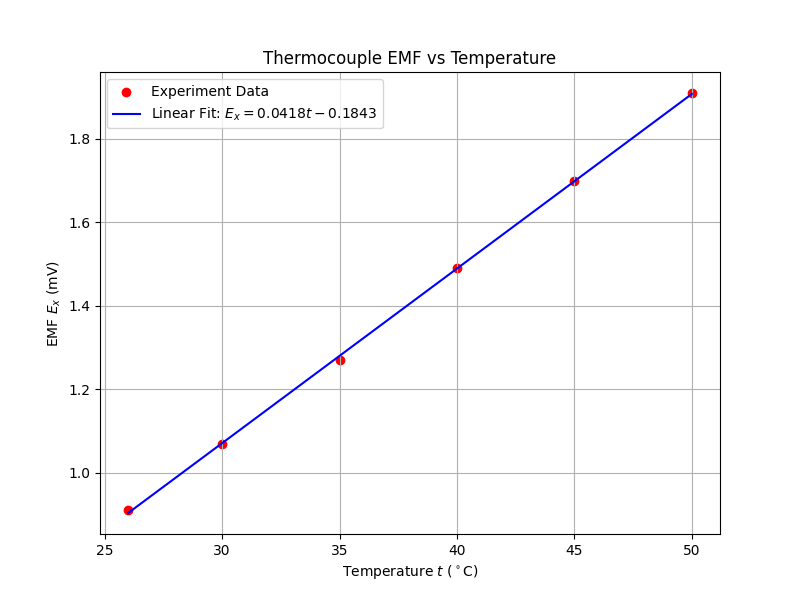
\includegraphics[width=0.7\textwidth]{thermocouple_plot.png}
    \caption{热电偶温差电动势 $E_x \sim t$ 曲线}
\end{figure}

\noindent
利用最小二乘法对实验数据进行线性拟合，设拟合方程为 $E_x = \alpha t + b$。
计算得到斜率 $\alpha \approx 0.04184 \ \mathrm{mV}/^\circ\mathrm{C}$，截距 $b \approx -0.18426\ \mathrm{mV}$，相关系数 $R^2 \approx 0.99979$。
因此，热电偶的温差电系数为 $\alpha = 0.04184 \ \mathrm{mV}/^\circ\mathrm{C}$。

\subsection{平衡电桥测铜电阻温度特性曲线}


\vspace{1em}

\noindent
室温：$t = 26.0\ ^\circ\mathrm{C}$ \hfill
电阻：$R_x = 56.0\ \Omega$

\begin{table}[h]
    \centering
    \begin{tabular}{lccccc}
        \toprule
        温度 $t$ ($^\circ\mathrm{C}$) & 30 & 35 & 40 & 45 & 50 \\
        \midrule
        电阻 $R_x$ ($\Omega$) & 57.5 & 58.7 & 59.8 & 61.0 & 62 \\
        \bottomrule
    \end{tabular}
\end{table}

\begin{figure}[H]
    \centering
    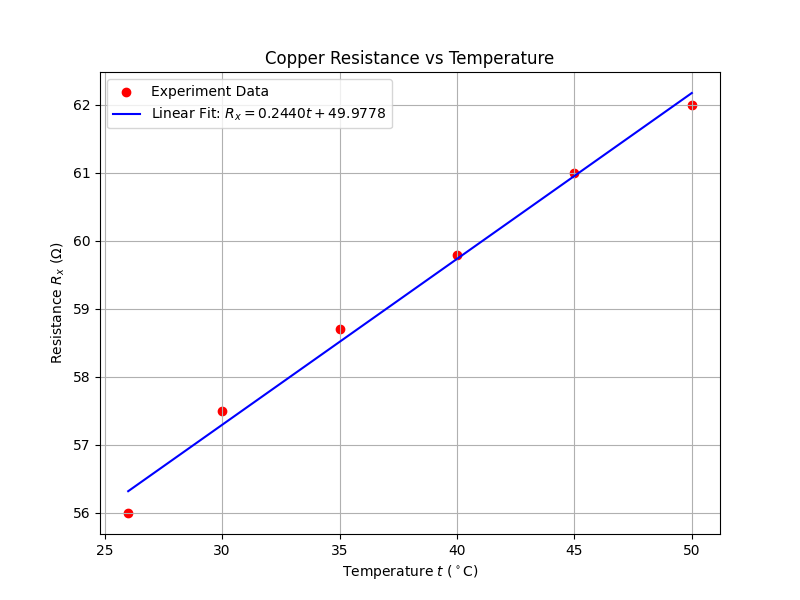
\includegraphics[width=0.7\textwidth]{bi_copper_resistance_plot.png}
    \caption{铜电阻温度特性 $R_x \sim t$ 曲线}
\end{figure}

\noindent
利用最小二乘法对实验数据进行线性拟合，设拟合方程为 $R_x = R_0 (1 + \alpha t) = R_0 + R_0 \alpha t$。
线性回归方程为 $R_x = k t + b$，得到斜率 $k \approx 0.24395\ \Omega/^\circ\mathrm{C}$，截距 $b = R_0 \approx 49.97782\ \Omega$。
相关系数 $R^2 \approx 0.99134$。
计算得铜电阻的温度系数 $\alpha = \frac{k}{b} \approx 4.88 \times 10^{-3} /^\circ\mathrm{C}$。

\subsection{非平衡电桥测热敏电阻特性曲线}

\vspace{1em}

\noindent
室温：$t = 26.0\ ^\circ\mathrm{C}$ \hfill
电阻：$R_t = 2.45\ \mathrm{k}\Omega$

\begin{table}[h]
    \centering
    \begin{tabular}{lccccc}
        \toprule
        温度 $t$ ($^\circ\mathrm{C}$) & 30 & 35 & 40 & 45 & 50 \\
        \midrule
        电阻 $R_t$ ($\mathrm{k}\Omega$) & 2.15 & 1.84 & 1.58 & 1.34 & 1.12 \\
        \bottomrule
    \end{tabular}
\end{table}

\begin{figure}[H]
    \centering
    \begin{minipage}{0.48\textwidth}
        \centering
        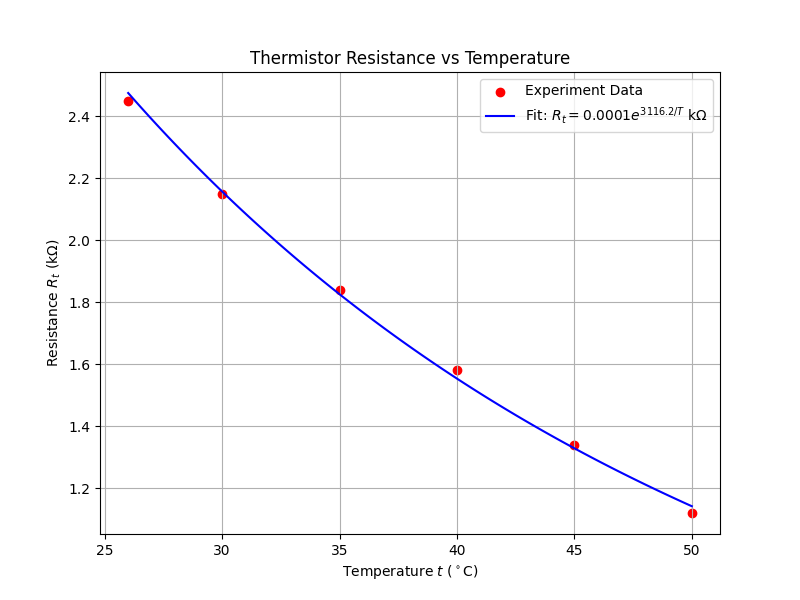
\includegraphics[width=\textwidth]{thermistor_resistance_plot.png}
        \caption{热敏电阻 $R_t \sim t$ 曲线}
    \end{minipage}
    \hfill
    \begin{minipage}{0.48\textwidth}
        \centering
        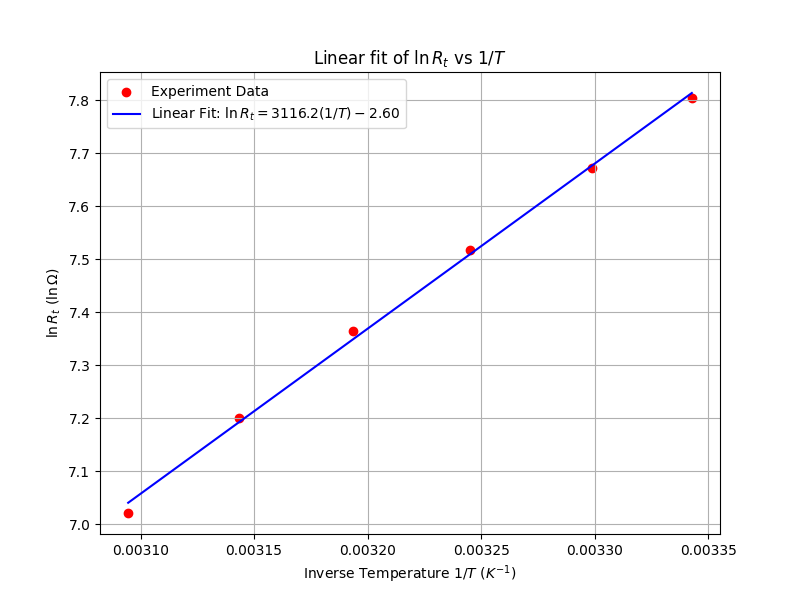
\includegraphics[width=\textwidth]{thermistor_ln_plot.png}
        \caption{$\ln R_t \sim 1/T$ 线性拟合曲线}
    \end{minipage}
\end{figure}

\noindent
根据热敏电阻的电阻温度特性公式 $R_t = A e^{B/T}$，两边取对数得 $\ln R_t = \ln A + \frac{B}{T}$。
令 $y = \ln R_t$，$x = 1/T$，则有线性关系 $y = Bx + \ln A$。
利用最小二乘法对实验数据进行线性拟合（注意将温度转换为开尔文温度 $T = t + 273.15$），得到斜率 $B \approx 3116.18\ \mathrm{K}$，截距 $\ln A \approx -2.60$（即 $A \approx 0.074\ \Omega$）。
相关系数 $R^2 \approx 0.99790$。
因此，该热敏电阻的材料常数 $B$ 值约为 $3116.18\ \mathrm{K}$。

\subsection{非平衡电桥热敏电阻温度计的设计}

\noindent
\textbf{1. 设计要求与参数选择：}

\noindent
设计温度区间：$30^\circ\mathrm{C} \sim 50^\circ\mathrm{C}$ \\
中心温度：$t_1 = 40^\circ\mathrm{C}$，即 $T_1 = 313.15\ \mathrm{K}$。 \\
热敏电阻特性常数（由4.3节拟合得）：$B \approx 3116.18\ \mathrm{K}$，$A \approx 0.074\ \Omega$。 \\
根据公式计算 $T_1$ 时的热敏电阻阻值：
\[
R_{xT1} = A e^{B/T_1} = 0.074 \times e^{3116.18/313.15} \approx 1.558\ \mathrm{k}\Omega = 1558\ \Omega
\]
设定线性输出目标方程：$U_o = \lambda + m(t - t_1)$ \\
选择表头参数：$\lambda = -400\ \mathrm{mV} = -0.4\ \mathrm{V}$，灵敏度 $m = -10\ \mathrm{mV}/^\circ\mathrm{C} = -0.01\ \mathrm{V}/^\circ\mathrm{C}$。

\vspace{1em}
\noindent
\textbf{2. 电桥参数计算：}

根据非平衡电桥的设计原理公式进行计算：

\noindent
(1) 工作电源电压 $E$：
\[
E = \left( \frac{4BT_1^2}{4T_1^2 - B^2} \right) m = \left( \frac{4 \times 3116.18 \times 313.15^2}{4 \times 313.15^2 - 3116.18^2} \right) \times (-0.01) \approx 0.969\ \mathrm{V}
\]
(注：若计算结果为负，取绝对值，实际电路中调整电源极性。此处计算值为理论参考，实际取值需考虑电源调节范围。)

\noindent
(2) 平衡臂电阻 $R_2$：
\[
R_2 = \frac{B - 2T_1}{B + 2T_1} R_{xT1} = \frac{3116.18 - 2 \times 313.15}{3116.18 + 2 \times 313.15} \times 1558 \approx 1035\ \Omega
\]

\noindent
(3) 桥臂比 $R_1/R_3$：
\[
\frac{R_1}{R_3} = \frac{2BE}{(B + 2T_1)E - 2B\lambda} - 1
\]
代入数值计算：
\[
\frac{R_1}{R_3} = \frac{2 \times 3116.18 \times 0.969}{(3116.18 + 626.3) \times 0.969 - 2 \times 3116.18 \times (-0.4)} - 1 \approx 0.125
\]
若取 $R_3 = 1000\ \Omega$ (固定)，则 $R_1 \approx 125\ \Omega$。

\vspace{1em}
\noindent
\textbf{3. 实际测量数据与特性曲线：}

\noindent
实际组装电桥参数：$R_3 = 1000\ \Omega$, $R_1 \approx 125\ \Omega$, $R_2 \approx 1035\ \Omega$, $E \approx 0.97\ \mathrm{V}$。

\begin{table}[h]
    \centering
    \caption{非平衡电桥热敏电阻温度计定标数据}
    \begin{tabular}{lccccc}
        \toprule
        设定温度 $t$ ($^\circ\mathrm{C}$) & 40.0 & 42.5 & 44.5 & 46.7 & 50.0 \\
        \midrule
        测试电压 $U_o$ ($\mathrm{mV}$) & -400 & -427 & -449 & -480 & -518 \\
        理论电压 ($\mathrm{mV}$) & -400 & -425 & -445 & -467 & -500 \\
        \bottomrule
    \end{tabular}
\end{table}

\begin{figure}[H]
    \centering
    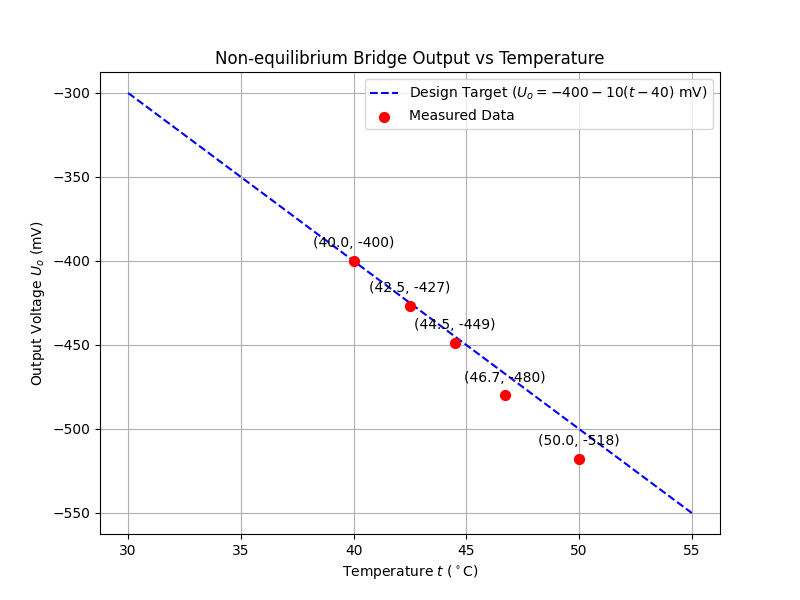
\includegraphics[width=0.7\textwidth]{thermometer_design_plot.png}
    \caption{非平衡电桥设计输出电压 $U_o \sim t$ 关系}
\end{figure}

\noindent
由图可见，设计的非平衡电桥在 $30 \sim 50^\circ\mathrm{C}$ 范围内输出电压 $U_o$ 与温度 $t$ 呈现良好的线性关系，且与设计目标 $U_o = -400 - 10(t - 40)\ (\mathrm{mV})$ 基本吻合，实现了将热敏电阻的非线性变化转化为电压的线性输出，可作为温度计使用。


\section{思考题}
\begin{enumerate}
    \item \textbf{为什么在低温实验中常用四线式伏安法测温度，而工业仪表中常用非平衡电桥测温度？}
    
    答：
    \begin{itemize}
        \item \textbf{低温实验中：} 常用的电阻温度计（如锗电阻、碳电阻等）在低温下可能会有较大的引线电阻或接触电阻变化，或者需要极高的测量精度。四线式伏安法（两根电流线，两根电压线）可以完全消除引线电阻和接触电阻对测量的影响。因为电压表输入阻抗极高，电流几乎不流过电压引线，测得的电压降精确反映了电阻元件两端的电压，从而精确测得电阻值。
        \item \textbf{工业仪表中：} 工业生产更注重实时性、连续测量及信号的转换传输。非平衡电桥可以将电阻的变化直接转化为电压信号输出，无需像平衡电桥那样反复调节平衡，适合自动记录和控制。虽然精度略逊于四线法，但结构简单、成本低，配合三线制接法已能满足大多数工业测温精度的要求。
    \end{itemize}

    \item \textbf{工业仪表中使用的三线式非平衡电桥测温度是怎么消除引线电阻的？}
    
    答：
    在三线制接法中，从测温电阻（如热电阻 $R_t$）引出三根导线，其中两根接在电桥的两个相邻桥臂上，第三根接在电源端。设三根导线电阻相等为 $r$。
    \begin{itemize}
        \item 将其中一根导线串联在热电阻 $R_t$ 所在的桥臂中。
        \item 将另一根导线串联在与 $R_t$ 相邻的比较桥臂（电阻为 $R_2$）中。
        \item 第三根导线接在电源回路中，对电桥的平衡状态无影响（仅分担极小一部分电源电压）。
    \end{itemize}
    当电桥平衡或计算非平衡电压时，由于两根引线分别位于电桥的相邻两臂，且材质、长度、温度环境相同（即电阻值 $r$ 相同），它们对电桥输出的影响大致相互抵消。例如在等臂电桥中，两臂电阻变为 $R_t+r$ 和 $R_2+r$，当 $R_t \approx R_2$ 时，电阻变化引起的电压输出受 $r$ 影响极小，从而有效消除了引线电阻及其随环境温度变化带来的测量误差。
\end{enumerate}

\section{原始数据和预习报告}

\begin{figure}[H]
    \centering
    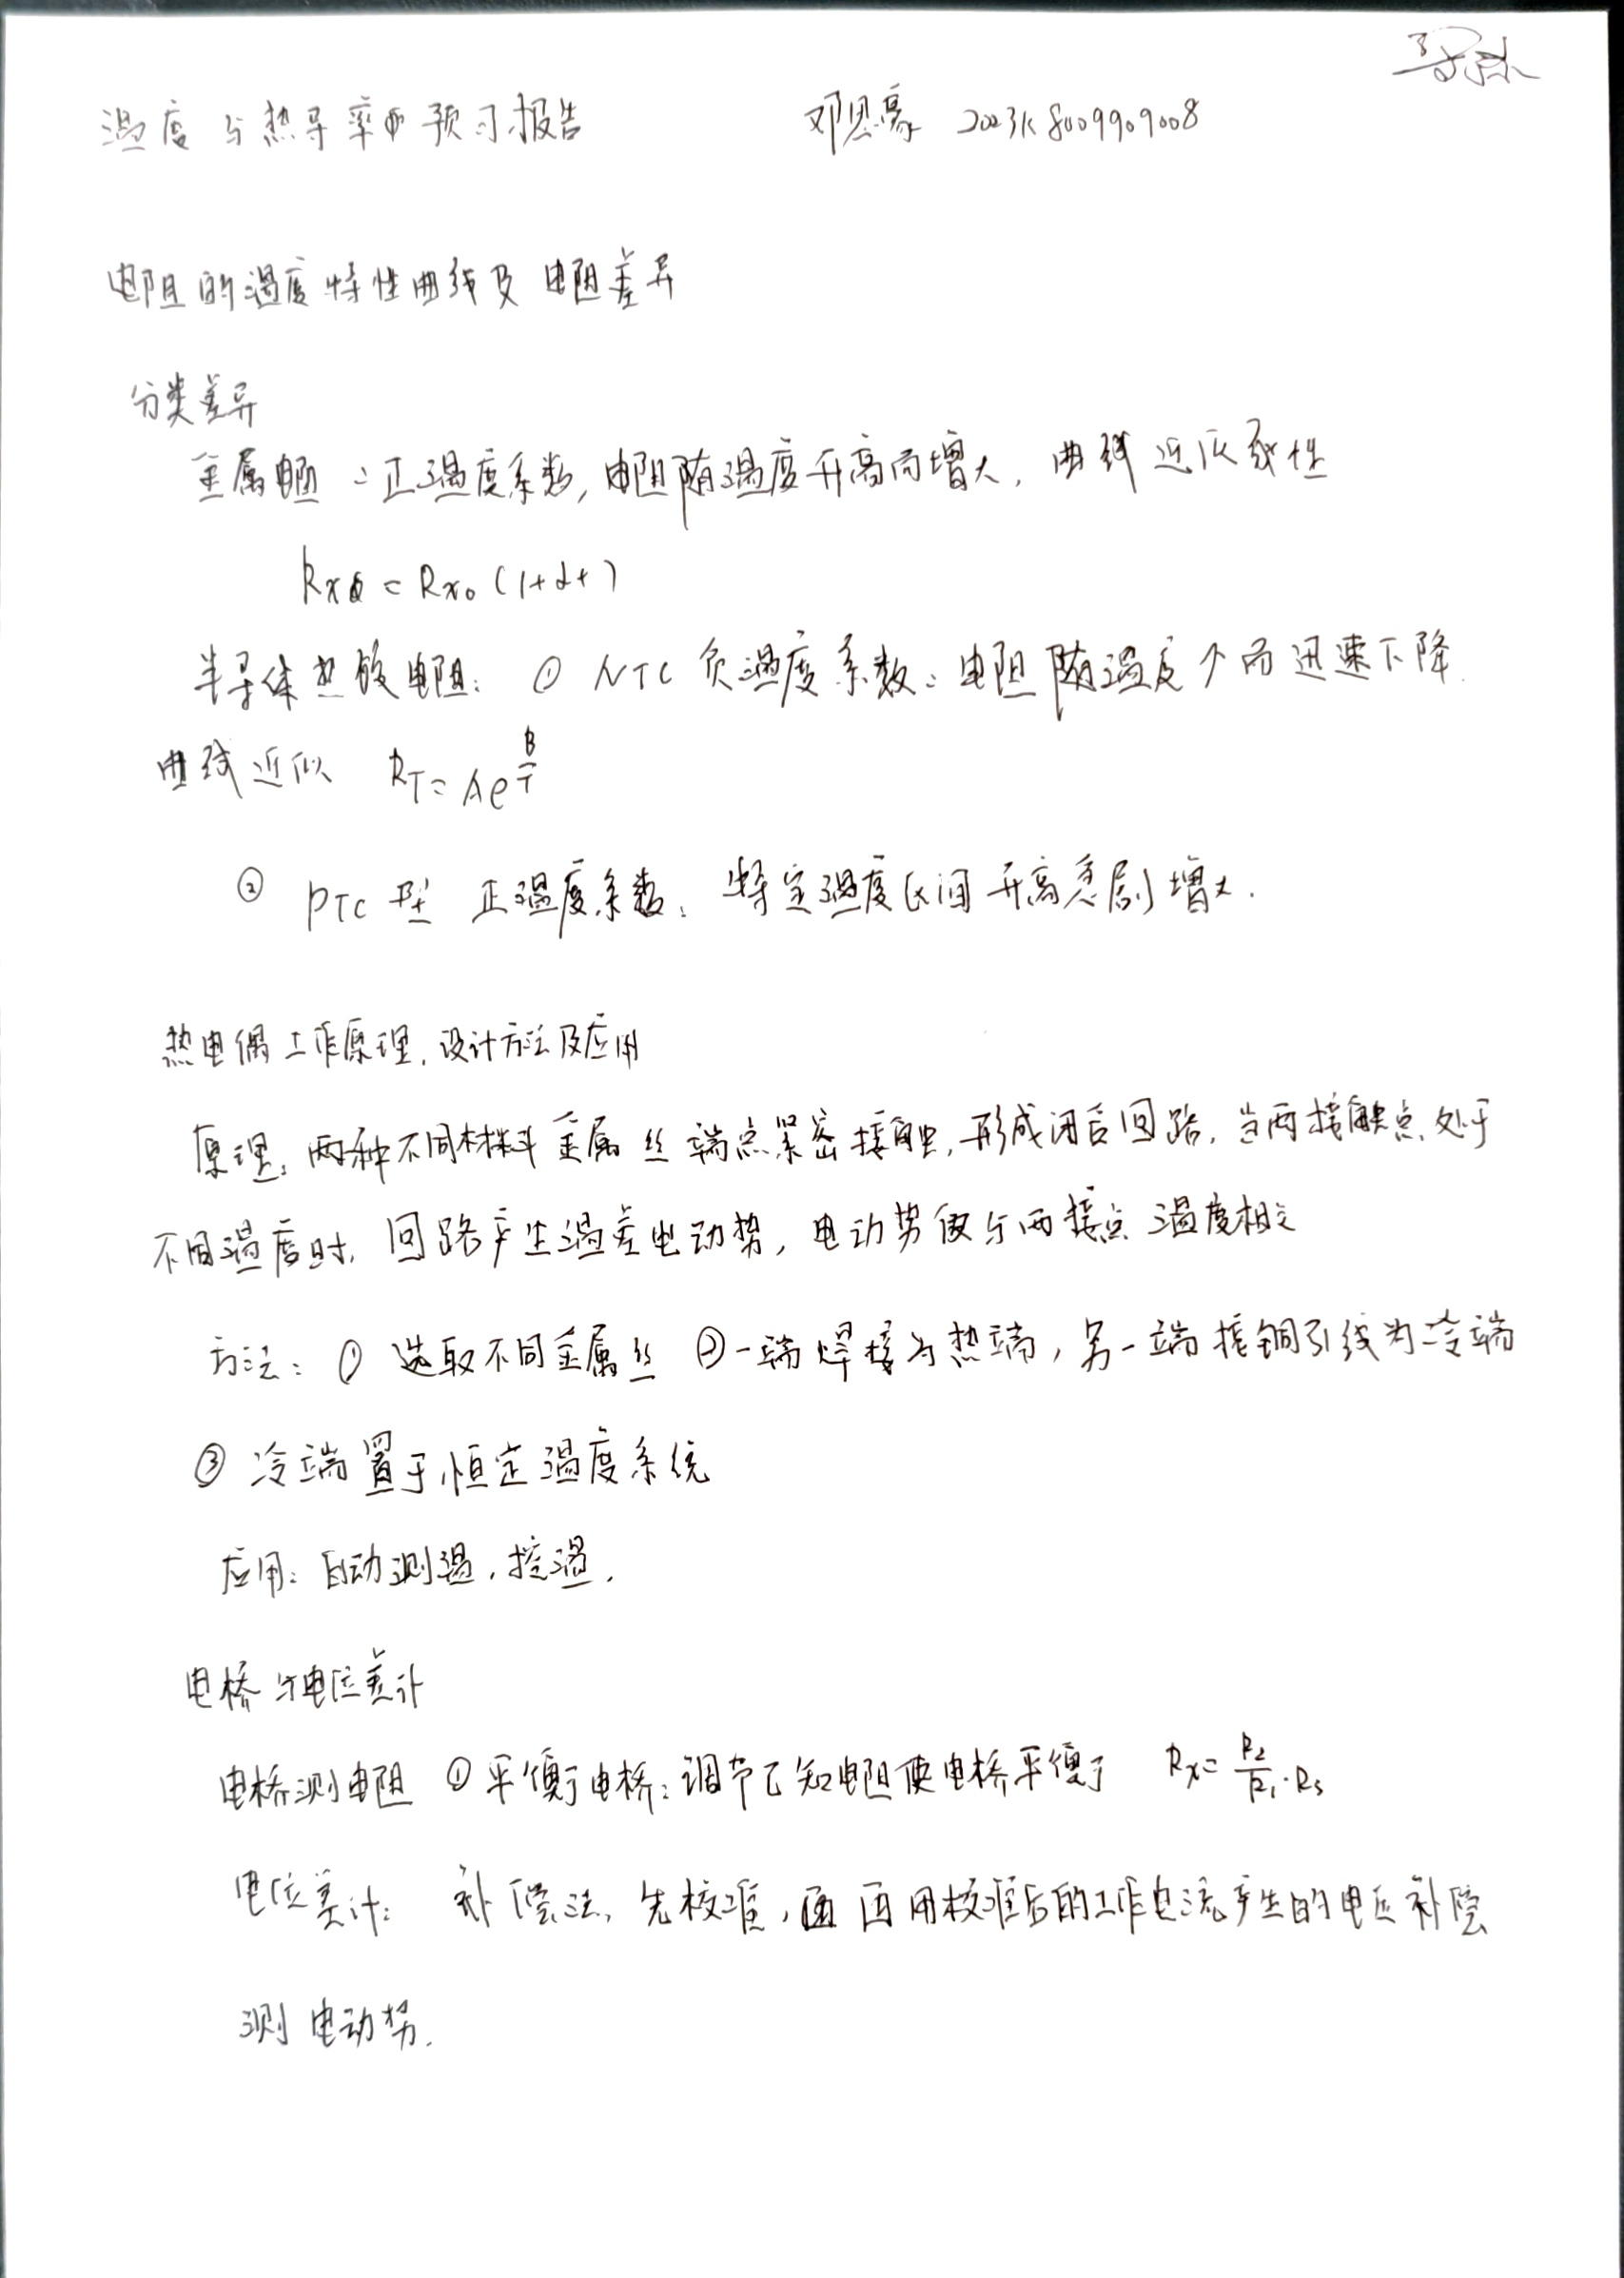
\includegraphics[width=0.9\textwidth]{record_raw.jpg}
\end{figure}

\begin{figure}[H]
    \centering
    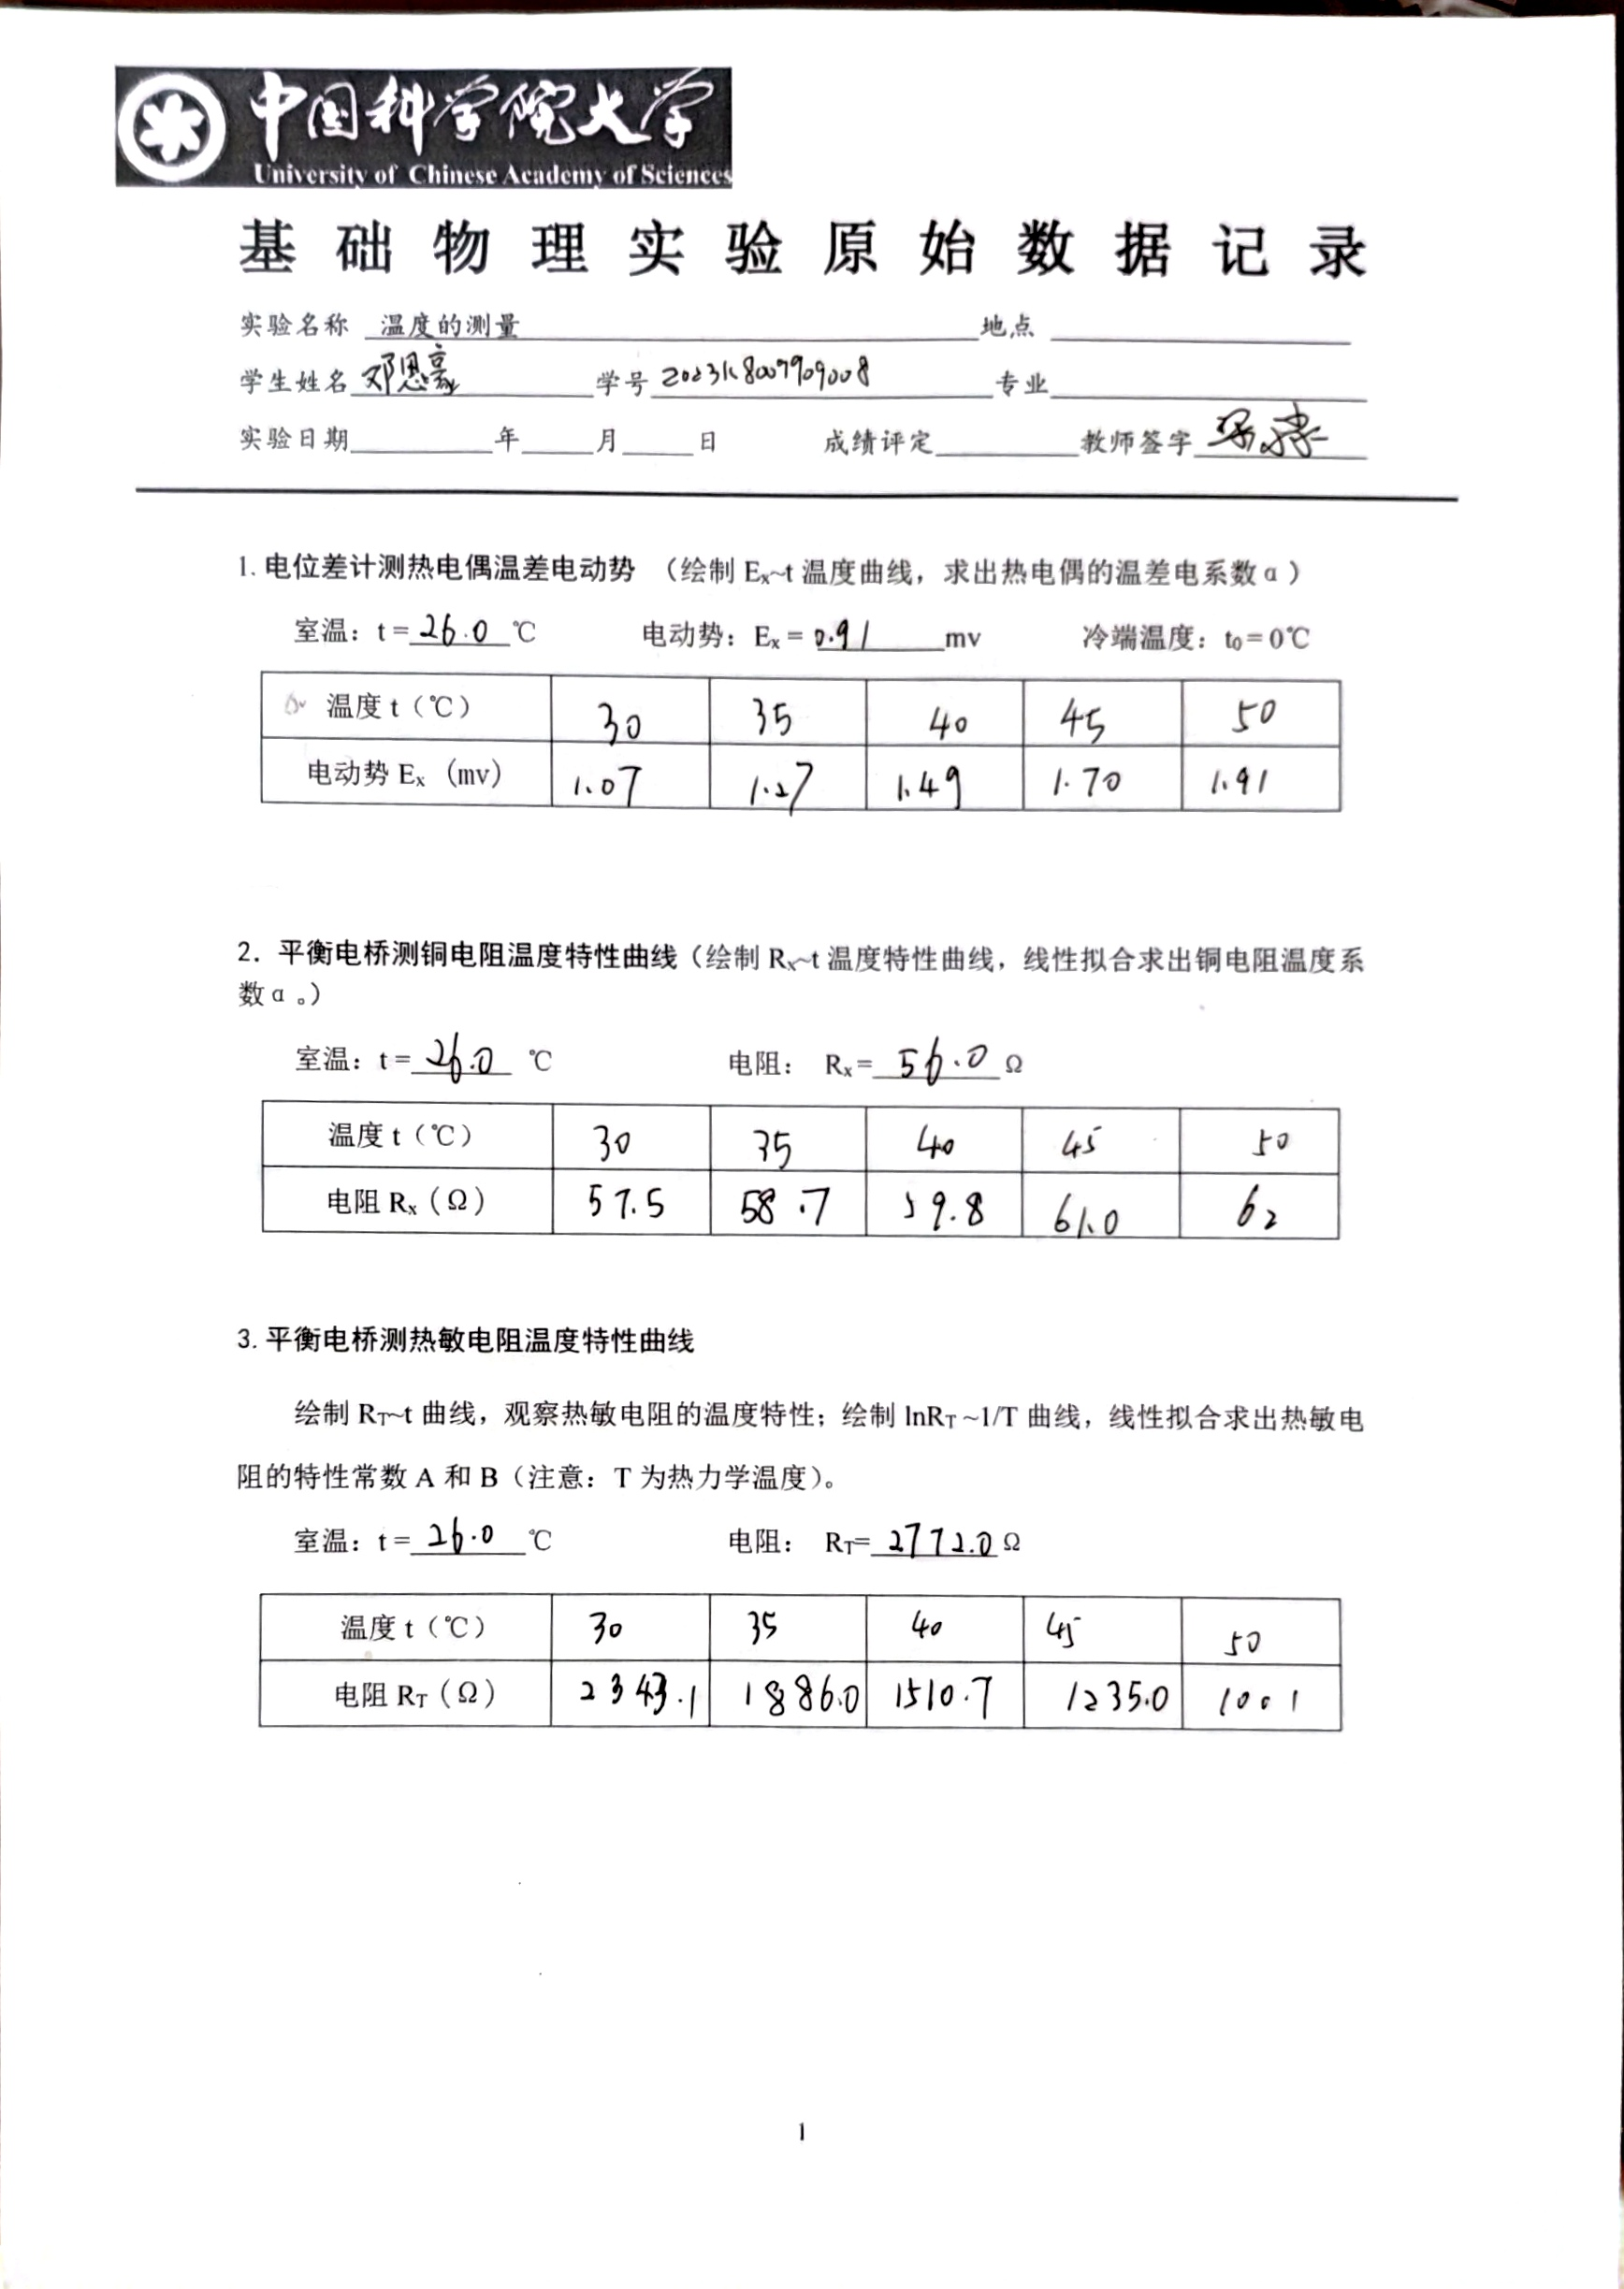
\includegraphics[width=0.9\textwidth]{record_raw1.jpg}
\end{figure}

\begin{figure}[H]
    \centering
    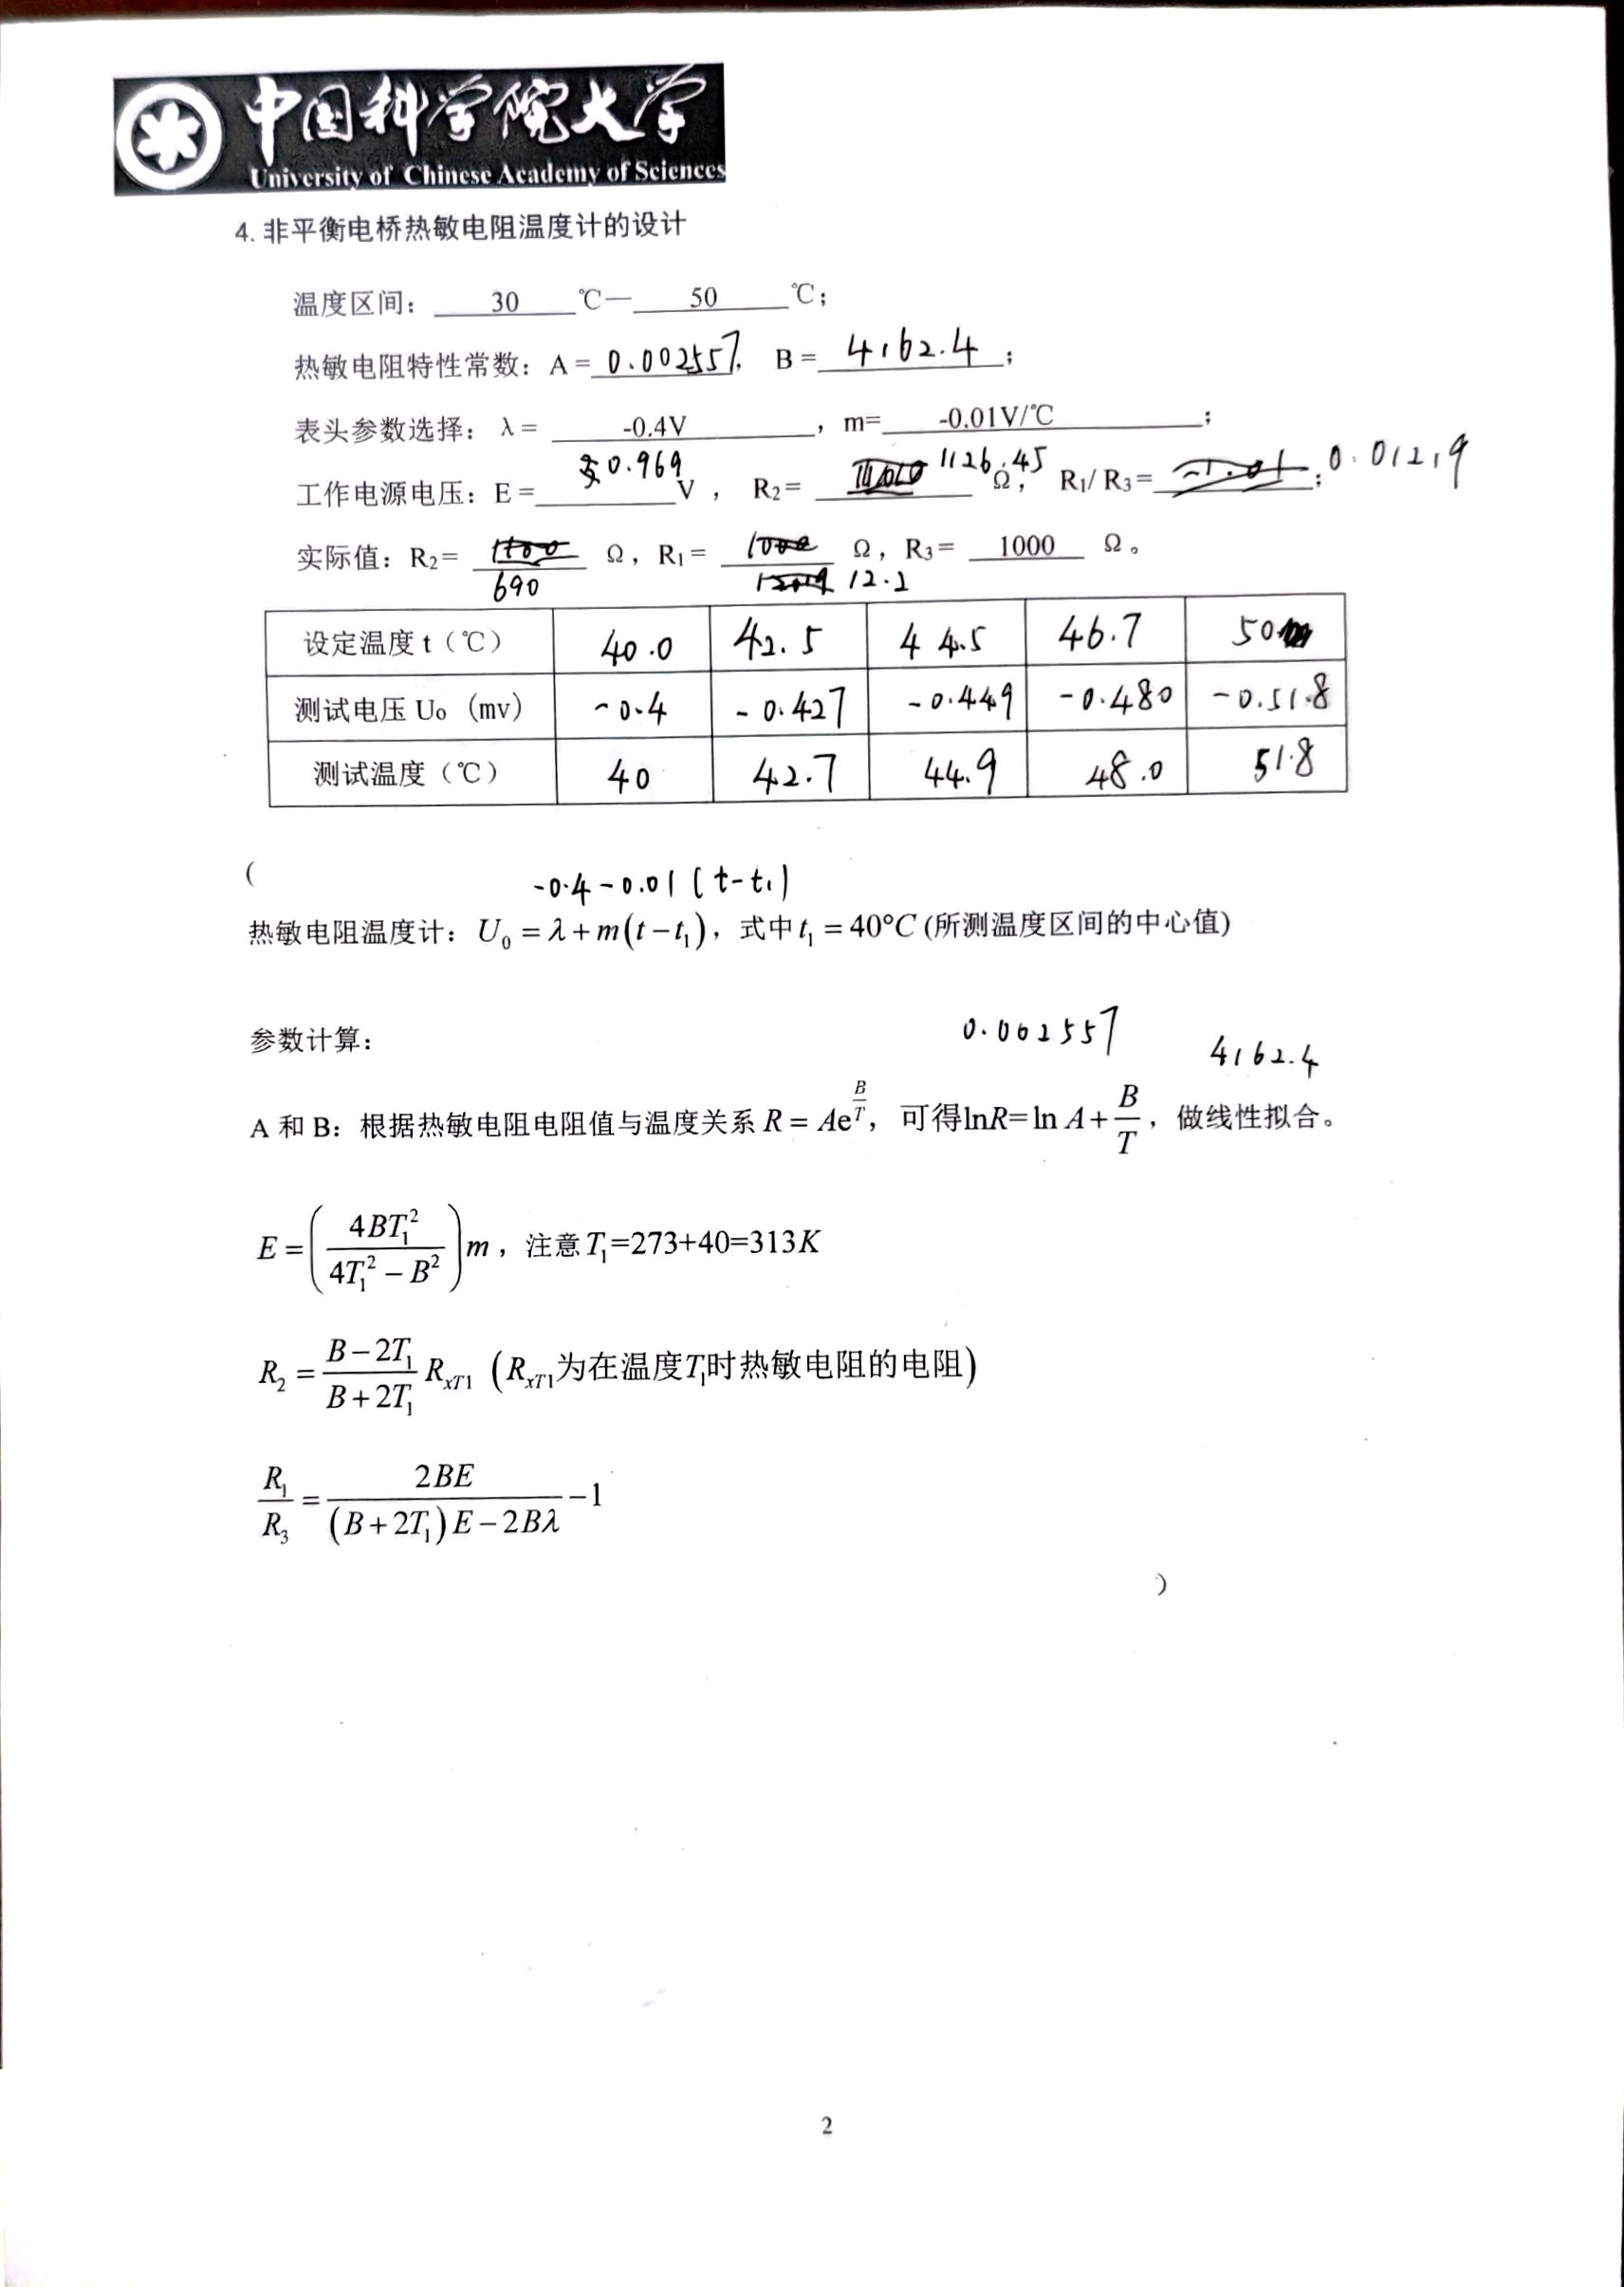
\includegraphics[width=0.9\textwidth]{record_raw2.jpg}
\end{figure}

\end{document}